\documentclass[letterpaper]{article} % DO NOT CHANGE THIS
\usepackage[submission]{aaai2027}  % DO NOT CHANGE THIS
\usepackage{times}  % DO NOT CHANGE THIS
\usepackage{helvet}  % DO NOT CHANGE THIS
\usepackage{courier}  % DO NOT CHANGE THIS
\usepackage[hyphens]{url}  % DO NOT CHANGE THIS
\usepackage{graphicx} % DO NOT CHANGE THIS
\urlstyle{rm} % DO NOT CHANGE THIS
\def\UrlFont{\rm}  % DO NOT CHANGE THIS
\usepackage{natbib}  % DO NOT CHANGE THIS AND DO NOT ADD ANY OPTIONS TO IT
\usepackage{caption} % DO NOT CHANGE THIS AND DO NOT ADD ANY OPTIONS TO IT
\frenchspacing  % DO NOT CHANGE THIS
\setlength{\pdfpagewidth}{8.5in} % DO NOT CHANGE THIS
\setlength{\pdfpageheight}{11in} % DO NOT CHANGE THIS

\usepackage{amsmath}
\usepackage{amssymb}
\usepackage{amsfonts}
\usepackage{booktabs}
\usepackage{array}
\usepackage{algorithm}
\usepackage{algorithmic}

\pdfinfo{
/TemplateVersion (2027.1)
}
\setcounter{secnumdepth}{0}

\newcommand{\method}{\textsc{TA-DVFG}}
\newcommand{\Gc}{\mathcal{G}_c}
\newcommand{\Ec}{\mathcal{E}_c}
\newcommand{\Ni}{\mathcal{N}_i}
\newcommand{\R}{\mathbb{R}}
% Leakage-safe MovieLens 1M rerun values.
% Update generated values here rather than hand-editing main text.
\newcommand{\BestSingleMovieAUC}{0.7402}
\newcommand{\TADVFGMovieAUC}{0.7516}
\newcommand{\FullMeshMovieAUC}{0.7497}
\newcommand{\AdaptivePairMovieAUC}{0.7510}
\newcommand{\TopKMovieAUC}{0.7487}
\newcommand{\TADVFGMovieCommM}{3.20M}
\newcommand{\FullMeshMovieCommM}{10.00M}
\newcommand{\AdaptivePairMovieCommM}{5.20M}
\newcommand{\TopKMovieCommM}{0.80M}
\newcommand{\PoneParams}{651,970}
\newcommand{\PtwoParams}{130,402}
\newcommand{\PthreeParams}{162}
\newcommand{\PfourParams}{825,218}
\newcommand{\PfiveParams}{297,938}
\newcommand{\ConsensusSteps}{1}
\newcommand{\GlobalTopK}{5}
\newcommand{\EdgeBudget}{15}
\newcommand{\MaxDegree}{2}
\newcommand{\MinEdges}{5}
\newcommand{\MinGain}{0.001}
\newcommand{\TopologyInterval}{20}
\newcommand{\PredictionSelfWeight}{0.85}


\title{Collaboration without Representation Alignment: Sparse Prediction Topology Learning for Vertical Graph Views}

\author{Anonymous Submission}
\affiliations{}

\begin{document}
\maketitle

\begin{abstract}
AI models increasingly operate as distributed components with different
architectures and internal representations. Vertical Federated Graph Learning
(VFGL) provides a concrete setting: parties hold private graph views over
aligned entities, yet existing methods often collaborate through intermediate
representations. This is restrictive when local predictors lack a compatible
latent interface. We instead collaborate through task-compatible output
distributions while keeping internal representations local.

Prediction space determines what can be shared; topology determines which
predictors participate and where their predictions can flow. We formulate this
as sparse peer-to-peer topology learning and propose \method{}. Using held-out
validation predictions, an active party evaluates candidate graphs by
post-consensus deployment performance. At inference, parties exchange class
distributions only over selected links and perform reliability-aware consensus.
The topology can target active-party, party-local, or joint readouts.

Across six controlled 15-party HGB-derived settings, \method{} outperforms Full
Mesh and matched sparse P2P controls with only 5--5.8 of 105 possible links.
The strongest centralized reference, Global Top-$k$, is numerically higher in
four settings and lower in two; with five seeds, paired tests do not resolve a
difference. This boundary is central: same-cardinality subset selection is
cheaper and slightly stronger for active-only readout, whereas sparse peer
exchange raises party-local accuracy by 1.85/2.67 points on ACM/DBLP Hard and
connected-party accuracy by 4.79/7.16 points. On MovieLens, \method{} reaches
0.7516 AUC with 3.20M transmitted scalars, versus 0.7497 and 10.00M for Full
Mesh. Thus, learned topology is not claimed to be necessary for one centralized
aggregate; its distinct role is party-local or joint deployment. \method{} is
an inference-stage collaboration mechanism rather than a formal privacy
mechanism or a fully serverless, end-to-end VFGL protocol.
\end{abstract}

\section{Introduction}

AI models increasingly operate as distributed components across devices,
organizations, and autonomous agents, where they may be developed independently
with different data, architectures, and internal representations. Collaboration
therefore cannot always assume homogeneous models or a jointly designed
interface. Vertical Federated Graph Learning (VFGL) provides a concrete setting
for this problem: parties hold different private feature blocks or graph views
over aligned entities and seek to collaborate without pooling those data.

Most VFGL methods combine graph information through intermediate
representations by exchanging, projecting, aggregating, or jointly optimizing
hidden states. Such mechanisms are natural when participants expose compatible
interfaces, but become restrictive for independently maintained predictors.
One party may use a GCN on an interaction graph, another a heterogeneous graph
encoder, and a third a non-graph predictor. Their latent spaces
$\mathcal{H}_1,\ldots,\mathcal{H}_N$ may differ in dimension and semantics, so
equal dimensionality alone does not establish alignment.

A shared latent space is not necessary, however, when parties solve the same
task for aligned targets. Their internal representations may be incompatible
while their outputs remain directly comparable:
\[
h_i\in\mathcal{H}_i,
\qquad
p_i\in\Delta^C.
\]
Prediction space determines \emph{what can be shared}; topology determines
\emph{which predictors participate and where their predictions can flow}. We therefore ask:
\begin{center}
\emph{Can heterogeneous predictors over vertical graph views collaborate
directly in prediction space without first aligning their hidden
representations?}
\end{center}

A common output space does not, however, make unrestricted exchange desirable.
Predictors differ in reliability and complementarity, so Full Mesh
communication can propagate weak predictions while incurring unnecessary cost.
Moreover, deployment may require an active-party readout, party-local
predictions, or a trade-off between them. Direct subset selection can suffice
for active-only readout, whereas party-local improvement requires useful peer
communication. For example, a hospital consortium may need both a registry-level aggregate
score and improved local predictions without exporting hidden states or routing
every inference through a permanent center. Similar dual-output requirements can
arise in multi-bank fraud screening. The problem is therefore to learn a sparse
graph whose utility is judged by deployment performance.

We propose \method{}, a validation-assisted sparse topology learner for trained
heterogeneous predictors. A label-holding active party uses held-out validation
predictions to estimate predictor reliability and evaluates each feasible
one-edge extension only after rerunning consensus over the entire tentative
graph. Beneficial links are greedily retained under edge-budget and degree
constraints. At inference time, parties exchange class distributions only
along the selected links and perform reliability-aware consensus. The topology
can be optimized for active-party, party-local, or joint deployment objectives,
and may leave weak predictors isolated when connecting them is not beneficial.
Topology selection is centralized, whereas deployment communication is
peer-to-peer over the learned graph.

\method{} operates on trained local predictors and does not prescribe a common
training algorithm. We evaluate the collaboration mechanism through two
complementary experimental tracks. Controlled HGB-derived settings isolate
topology-selection behavior under known mixtures of useful and weak graph-view
predictors. MovieLens provides a real-data recommendation benchmark with
heterogeneous private views and predictor families.

Our contributions are:
\begin{itemize}

\item We formulate a model-heterogeneous collaboration setting for vertical
graph views in which trained local predictors share task-level outputs without
requiring a common hidden-state interface.

\item We propose validation-assisted sparse topology learning that evaluates
candidate links through their effect on whole-graph post-consensus deployment
performance rather than through edge-local scores.

\item We support active-party, party-local, and joint deployment objectives
and separate participant-selection effects from peer-exchange effects.

\item We evaluate the method across controlled HGB and heterogeneous
MovieLens settings, covering communication, label ownership, scalability,
deployment objectives, and a five-seed frozen-predictor latent-alignment study.

\end{itemize}

\section{Related Work}

\paragraph{Vertical federated graph learning.}
VFGL methods such as VFGNN \cite{chen2022vfgnn}, FedVGCN
\cite{ni2021fedvgcn}, VerFedGNN \cite{mai2023verfedgnn}, and GLASU
\cite{zhang2023glasu} study how graph information can be combined across
vertically partitioned parties. These methods differ in architecture and
optimization, and may permit party-specific local encoders, but collaboration
is typically coordinated through intermediate representations, shared
computation, or jointly optimized fusion mechanisms. Our setting addresses a
different interface assumption: local predictors need not expose hidden states
that are designed for cross-party combination.

\paragraph{Model-heterogeneous federated learning.}
Model-heterogeneous FL relaxes the requirement that participants use identical
models. FedHM \cite{yao2025fedhm} accommodates different model capacities,
Flex-VFL \cite{castiglia2024flexvfl} supports heterogeneous vertical
participants within a coordinated optimization framework, and VFedMH
\cite{wang2023vfedmh} jointly trains multiple heterogeneous models through
aggregated embeddings. These approaches make heterogeneous models
collaborative by constructing a parameter-, optimization-, or
representation-level coordination interface. In contrast, \method{} treats
heterogeneous predictors as persistent local components that need not share
architectures, hidden dimensions, or latent semantics. Their hidden states are
neither aligned nor exchanged; collaboration begins only after each predictor
maps its private input to a compatible task-output space.

\paragraph{Prediction-level collaboration.}
FedMD \cite{li2019fedmd}, FedDF \cite{lin2020feddf}, and FedGen
\cite{zhu2021fedgen} show that model outputs can mediate collaboration among
heterogeneous models. Their primary goal is knowledge transfer, model fusion, or
distillation through public data, a server model, or generated knowledge.
In contrast, \method{} treats predictions as inference-time messages and
directly learns the sparse peer-to-peer communication graph.

\paragraph{Ensemble selection and expert combination.}
Classical stacking learns a meta-level combiner
\cite{wolpert1992stacked}, ensemble selection chooses predictor subsets
\cite{caruana2004ensemble}, and mixtures of experts learn gating rules
\cite{jacobs1991moe}. \method{} does not claim novelty for predictor selection
itself. Instead, it returns a sparse communication graph, scores candidate edges
after rerunning whole-graph consensus, and may optimize party-local
post-consensus states rather than one centralized ensemble output.

\paragraph{Decentralized and adaptive topology.}
Decentralized optimization exchanges model parameters over a client graph
\cite{lian2017dpsgd}; SpreadGNN \cite{he2022spreadgnn} and Lumos
\cite{pan2023lumos} study non-vertical federated graph settings, while
De-VertiFL \cite{huertas2024devertifl} and semi-decentralized vertical
optimization \cite{valdeira2023mtcd} adopt different communication and training
interfaces. Adaptive methods cluster or match clients
\cite{sattler2020clustered,li2022panm}, while federated graph methods can also
construct collaboration graphs
\cite{zhong2024spreadfgl,guo2025dfedsst}. Our criterion is different: a
candidate link is inserted into the current graph, consensus is rerun, and the
resulting deployment readout is evaluated. Edge utility is defined by its effect within the current topology and
objective, not by a precomputed pairwise score.

\begin{table}[t]
\centering
\scriptsize
\setlength{\tabcolsep}{2.5pt}
\caption{Interface-level positioning. ``Local consensus'' denotes explicit
optimization of party-local post-consensus states rather than generic local
inference after training.}
\label{tab:positioning}
\begin{tabular}{lcccc}
\toprule
Approach & Shared latent & Prediction & Learned P2P & Local consensus \\
 & interface & messages & topology & objective \\
\midrule
VFGL fusion & Yes & No & No & No \\
FedMD-style & No & Yes & No & No \\
Centralized latent fusion & Yes & No & No & No \\
Global Top-$k$ & No & Yes & No & No \\
\method{} & \textbf{No} & \textbf{Yes} & \textbf{Yes} & \textbf{Yes} \\
\bottomrule
\end{tabular}
\end{table}

Table~\ref{tab:positioning} highlights the intended gap. Prediction-level
compatibility removes the need for a shared latent interface, but does not by
itself define peer communication paths or optimize party-local post-consensus
states. Centralized latent fusion provides a stronger-information interface when
genuine hidden states can be collected and projected, but does not produce a
sparse peer-to-peer deployment graph. \method{} instead makes this graph the
object of collaboration.

\section{Problem Setup}

Let $\mathcal{P}=\{1,\ldots,N\}$ denote parties that describe the same
aligned target set $V$. Party $i$ privately holds
\[
G_i=(V,X_i,A_i),
\]
where $X_i\in\mathbb{R}^{|V|\times d_i}$ is a private feature block and
$A_i$ is a private graph or relation view. Its predictor is
\begin{equation}
H_i=\phi_i(X_i,A_i), \qquad
P_i=\operatorname{softmax}(\psi_i(H_i)),
\label{eq:local_predictor}
\end{equation}
where $H_i\in\mathcal{H}_i$ may lie in a party-specific latent space and
$P_i[v]\in\Delta^C$ is a class distribution for target $v$. We assume
aligned targets, a shared task, and compatible output semantics, but not a
common encoder family, hidden dimension, or latent coordinate system. We do not require identical raw-confidence scales for reliability ranking:
predictor reliability is estimated from held-out validation performance rather
than from raw confidence alone. This weighting is not a per-party calibration
procedure.

Let $G_c=(\mathcal{P},E_c)$ be an undirected candidate communication graph.
A selected edge set $E\subseteq E_c$ determines which parties can directly
exchange predictions, with
\[
\mathcal{N}_i(E)=\{j:(i,j)\in E\}.
\]
Raw features, graph structures, model parameters, and hidden states remain
local. The selected graph need not be connected: isolating an unhelpful
predictor may be preferable to forcing every party into a shared connected
component.

Given topology-validation targets $V_{\mathrm{topo}}$, we seek
\begin{equation}
E^\star=
\arg\max_{\substack{
E\subseteq E_c,\ |E|\le B\\
\deg_E(i)\le d_{\max},\ \forall i
}}
s(E),
\label{eq:topology_objective}
\end{equation}
where $s(E)$ is the deployment score measured after prediction consensus over
the entire topology $E$. The budget $B$ is an upper bound; $m$, introduced
below, is a separate minimum quota. Test labels are never used for local
training, topology selection, reliability estimation, or model selection.

\section{Method}

\paragraph{Reliability-aware consensus.}
Let $\mathcal{M}$ denote the task-level validation metric: classification
accuracy for HGB and ROC-AUC for MovieLens. For each party $i$, the active
party estimates validation reliability as
\begin{equation}
r_i =
\mathcal{M}\!\left(
P_i[V_{\mathrm{topo}}],
y_{V_{\mathrm{topo}}}
\right),
\qquad
\bar r_i=\max(r_i,10^{-3}).
\label{eq:reliability}
\end{equation}
Reliability determines message weights but does not directly determine which
edges are selected. The implemented reliability exponent is $1.0$. For each
non-isolated party, define
\begin{equation}
\alpha_{ij}(E) =
\frac{\bar r_j}
{\sum_{\ell\in\mathcal{N}_i(E)}\bar r_\ell},
\qquad
j\in\mathcal{N}_i(E).
\label{eq:consensus_weight}
\end{equation}
Starting from $P_i^{(0)}=P_i$, the consensus update is
\begin{equation}
P_i^{(k+1)}(E)
=
\eta P_i^{(k)}(E)
+
(1-\eta)
\sum_{j\in\mathcal{N}_i(E)}
\alpha_{ij}(E)P_j^{(k)}(E),
\label{eq:consensus}
\end{equation}
with isolated parties retaining their current predictions. By default, we use
$\eta=0.85$ and one consensus step. The same operator is applied to cached
validation predictions during topology selection and to predictions over
$E^\star$ at inference time. Because all exchanged objects lie in
$\mathbb{R}^C$, consensus remains well defined regardless of the parties'
private latent spaces. Implementation details and proofs are provided in the
supplementary material.

\paragraph{Deployment readouts.}
After $K$ consensus steps, party-local deployment directly uses
$P_i^{(K)}(E)$. For active-party deployment, the implementation reads out the
non-isolated parties,
\[
S(E)=\{i:\deg_E(i)>0\},
\]
and falls back to all parties only for the edgeless topology. The active party
has no additional special term. For $i\in S(E)$, define
\begin{equation}
\begin{aligned}
\omega_i(E)
&=
\bar r_i\bigl(\deg_E(i)+1\bigr)^{1/2},
\\
Q_{\mathrm{active}}(E)
&=
\sum_{i\in S(E)}
\frac{\omega_i(E)}
{\sum_{j\in S(E)}\omega_j(E)}
\\[-2pt]
&\qquad {}\times P_i^{(K)}(E).
\end{aligned}
\label{eq:active_readout}
\end{equation}
 Candidate graphs are evaluated by
\begin{align}
s_{\mathrm{active}}(E)
&=
\mathcal{M}(Q_{\mathrm{active}}(E),y), \\
s_{\mathrm{local}}(E)
&=
\frac{1}{N}
\sum_i
\mathcal{M}(P_i^{(K)}(E),y), \\
s_{\mathrm{joint}}(E)
&=
\lambda s_{\mathrm{active}}(E)
+
(1-\lambda)s_{\mathrm{local}}(E).
\label{eq:deployment_objectives}
\end{align}
All scores use only $V_{\mathrm{topo}}$, so deployment objectives can favor
distinct graphs.

\paragraph{Validation-assisted graph selection.}
Starting from $E=\varnothing$, the selector evaluates every feasible one-edge
extension $E\cup\{e\}$ that satisfies the edge-budget and degree constraints.
Each candidate is scored only after running Eq.~\eqref{eq:consensus} over the
entire tentative topology and applying the selected deployment objective
defined above. The best candidate edge is
\[
e^\star
=
\arg\max_{e\in\mathcal{F}(E)}
s(E\cup\{e\}).
\]
While fewer than $m$ edges have been selected, the best feasible edge is added
unconditionally. Thereafter, it is accepted only if
\[
s(E\cup\{e^\star\})-s(E)\ge\tau.
\]
For $m=0$, even the first edge must clear $\tau$, so an empty graph remains
feasible. Unlike pairwise matching, this scores each edge in the current
topology and deployment objective, even when its endpoints are not the strongest
pair in isolation. Global Top-$k$ instead ranks parties for centralized
collection without defining peer-to-peer paths.

\paragraph{Why whole-graph scoring matters.}
Edge utility is context dependent. Under the reported one-step consensus,
adding $(i,j)$ directly updates its endpoints, but the value of those updates
still depends on the current topology, the participating predictor set, and the
final active or local readout. A pairwise score computed before insertion
therefore need not predict the value of the same edge after it is placed in the
current graph. Instead, the selector evaluates the deployment consequence of
each feasible one-edge extension. For larger $K$, the same formulation also
captures multi-hop propagation.

\begin{algorithm}[t]
\caption{Validation-Assisted Sparse Topology Learning}
\label{alg:topology}
\begin{algorithmic}[1]
\REQUIRE Validation predictions $\{P_i\}$, reliabilities $\{r_i\}$,
score $s(\cdot)$, budget $B$, degree limit $d_{\max}$, minimum links $m$,
threshold $\tau$
\STATE $E\leftarrow\emptyset$, $q\leftarrow s(E)$
\WHILE{$|E|<B$}
    \STATE $\mathcal{F}(E)\leftarrow$ feasible one-edge extensions
    \IF{$\mathcal{F}(E)=\emptyset$}
        \STATE \textbf{break}
    \ENDIF
    \FORALL{$e\in\mathcal{F}(E)$}
        \STATE Run $K$-step consensus on $E\cup\{e\}$
        \STATE $q_e\leftarrow s(E\cup\{e\})$
    \ENDFOR
    \STATE $e^\star\leftarrow\arg\max_{e\in\mathcal{F}(E)} q_e$
    \IF{$|E|<m$ or $q_{e^\star}-q\geq\tau$}
        \STATE $E\leftarrow E\cup\{e^\star\}$; $q\leftarrow q_{e^\star}$
    \ELSE
        \STATE \textbf{break}
    \ENDIF
\ENDWHILE
\RETURN $E$
\end{algorithmic}
\end{algorithm}

Algorithm~\ref{alg:topology} makes the graph-level objective explicit. A
candidate edge is evaluated only after it has been inserted into the current
graph, consensus has been rerun, and the intended deployment readout has been
measured. Thus, $B$ remains an upper bound, while $m$ controls only the
initial minimum quota.

\paragraph{Selection complexity.}
The greedy search accepts at most $B$ edges and, in the worst case, evaluates
$O(B|E_c|)$ candidate graph extensions. With cached predictions, a direct
implementation costs
\[
O(B|E_c|K|V_{\mathrm{topo}}|C),
\]
up to readout costs and sparse-graph constants, whereas deployment traffic
scales with $|E^\star|$ rather than $|E_c|$. Candidate evaluation, rather than
sparse inference, is therefore the current scalability bottleneck; the
party-count study measures this cost directly.

\paragraph{Basic properties.}
The consensus operator in Eq.~\eqref{eq:consensus} is row-stochastic. It
therefore preserves valid class distributions, remains independent of private
latent spaces, and limits information after $K$ steps to parties within $K$
graph hops. The greedy selector is feasible by construction and terminates
after at most $B$ accepted edge additions. Full proofs and the sparse
communication bound are provided in the supplementary material.

\paragraph{Protocol and communication boundary.}
\method{} operates on trained local predictors and does not prescribe a common
training algorithm. We also evaluate a label-siloed variant in which only the
active party receives labels; passive parties send train-node logits and
receive logit-space gradients. This experiment tests label ownership rather
than formal privacy. For $M$ inference targets and $K$ consensus steps,
peer-to-peer exchange over an undirected topology costs
\[
2|E^\star|KMC
\]
transmitted scalars, compared with
\[
N(N-1)KMC
\]
for Full Mesh. Detailed training, communication, and proof material is provided
in the supplementary material.

For active-readout experiments, deployment communication is reported as the sum
of peer exchange and readout collection, while low-frequency topology-control
traffic is accounted for separately. We report numerical communication costs
rather than relying only on asymptotic edge counts.

\section{Experiments}
\label{sec:experiments}

\begin{table*}[!t]
\centering
\footnotesize
\setlength{\tabcolsep}{3.1pt}
\caption{HGB Test@BestVal accuracy (\%, mean $\pm$ SD over five seeds).
Global Top-$k$ is higher than \method{} in four settings and lower in two.
Oracle Matched is a diagnostic post-hoc envelope over matched sparse controls;
bold/underline denote best/second-best.}
\label{tab:hgb-main}
\begin{tabular}{lcccccc}
\toprule
Method & ACM Main & ACM Hard & DBLP Main & DBLP Hard & IMDB Main & IMDB Hard \\
\midrule
Global Reliability & $86.06\pm2.29$ & $75.98\pm4.32$ & $90.96\pm0.52$ & $88.08\pm1.44$ & $28.51\pm0.76$ & $28.93\pm1.57$ \\
Global Top-$k$ & $\mathbf{89.82\pm1.01}$ & $\underline{85.50\pm2.78}$ & $\underline{91.43\pm0.65}$ & $\mathbf{90.57\pm1.04}$ & $\mathbf{39.27\pm0.87}$ & $\mathbf{30.44\pm0.92}$ \\
Oracle Matched & $76.97\pm7.58$ & $67.71\pm20.57$ & $88.48\pm3.95$ & $68.30\pm29.84$ & $29.74\pm0.97$ & $30.04\pm1.33$ \\
Full Mesh & $85.96\pm2.30$ & $75.52\pm5.04$ & $90.86\pm0.49$ & $88.01\pm1.45$ & $28.49\pm0.77$ & $29.03\pm1.33$ \\
\method{} & $\underline{89.52\pm1.71}$ & $\mathbf{85.54\pm2.91}$ & $\mathbf{91.50\pm1.37}$ & $\underline{90.25\pm1.14}$ & $\underline{38.65\pm0.86}$ & $\underline{30.08\pm0.97}$ \\
\bottomrule
\end{tabular}
\end{table*}


Our evaluation addresses five questions.
\textbf{Q1: Sparse topology.}
Does learned sparsity improve over dense, fixed matched-sparse, adaptive,
and centralized prediction-selection references?
\textbf{Q2: Heterogeneity.}
Does the approach transfer to real-data heterogeneous predictor interfaces?
\textbf{Q3: Mechanism.}
What does graph structure provide beyond direct participant selection and
pairwise adaptation?
\textbf{Q4: Deployment.}
Do different readout objectives prefer different topologies?
\textbf{Q5: Interface assumption.}
When genuine hidden states are available to a centralized fusion module, how
does sparse prediction-topology learning compare with reliability-selected
latent alignment?

\paragraph{Protocol.}
We use two complementary evaluation tracks. The controlled track contains
15-party HGB-derived ACM, DBLP, and IMDB settings \cite{lv2021hgb}.
Useful predictors are instantiated from dataset-specific relation or KNN graph
views. Controlled weak/noisy parties preserve the same aligned targets, labels,
and data split, but apply a seed-specific row permutation to the private feature
block, add zero-mean Gaussian noise with scale $1.0$, and replace the private
graph with an independently sampled random graph of configured degree $4$.
Main uses six useful and nine weak or noisy parties; Hard uses three useful and
twelve weak or noisy parties. Party identities are independently reshuffled for
each seed, and all methods receive identical cached local-prediction
trajectories.

The second track uses GroupLens MovieLens 1M (\texttt{ml-1m.zip})
\cite{harper2015movielens}. Targets are observed rating rows: ratings
$\ge4$ are positive, ratings $1$--$3$ are negative, and no negative sampling
or unobserved-pair negatives are used. Rows are ordered by
\texttt{(timestamp, user\_id, movie\_id)} and split chronologically
70/10/20; all fitted models and preprocessing statistics are train-only.
Five parties observe distinct private views and use independently designed
predictor families. Controlled 15-party Main and Hard variants further stress
the methods with many weak predictors. All experiments use seeds 42--46. HGB
reports Test@BestVal accuracy, whereas MovieLens reports ROC-AUC.

Global Top-$k$ is the strongest centralized prediction-selection reference.
Ring, Random, Expander, Adaptive Pairwise, Adaptive Complementarity, and Full
Mesh serve as P2P comparisons. Best Single is retained as the no-collaboration
reference for MovieLens, where it is evaluated under the same chronological
split. Oracle Matched in Table~\ref{tab:hgb-main} is a post-hoc test-mean upper
envelope over Ring, Random, and Expander and is therefore not a deployable
baseline.

Unless explicitly varied in a sensitivity study, the selector uses one
consensus step ($K=1$), edge budget $B=15$, maximum degree
$d_{\max}=2$, minimum link count $m=5$, gain threshold
$\tau=0.001$, and a 20-epoch topology update interval. Local predictors train
independently; each scheduled refresh uses held-out validation predictions to
update the topology without back-propagating through the selector, and inference
uses the current graph for prediction exchange and consensus. Global Top-$k$
uses $k=5$. The primary protocol uses the held-out validation split for
reliability estimation, candidate-topology scoring, and validation-based epoch
selection; test labels remain reserved for final reporting. We audited all 90
headline HGB result rows and verified that their resolved configurations matched
these defaults. The full audit is provided in the supplementary material.



\paragraph{Controlled HGB results and the active-only boundary.}
Table~\ref{tab:hgb-main} shows the boundary: Global Top-$k$ is numerically
higher in four settings and \method{} in two. Five-seed paired Wilcoxon tests
do not resolve a difference, which is neither evidence of equivalence nor of
superiority. We therefore do not claim that graph learning is necessary for one
centralized readout. Against P2P alternatives, however, \method{} outperforms
Full Mesh and the post-hoc Oracle Matched envelope in all six settings with only
5--5.8 of 105 links. The remaining question is whether peer topology adds value
when local parties also consume predictions.

IMDB is selection-dominated: non-selective methods cluster near 28--29\%,
whereas Global Top-$k$ and \method{} rise sharply on IMDB Main. We therefore
attribute this mainly to filtering harmful predictors, not graph structure
alone; explaining the larger useful/weak quality gap requires per-party
diagnostics.

\begin{table}[!t]
\centering
\scriptsize
\setlength{\tabcolsep}{2.8pt}
\caption{Active-only Hard-setting boundary. Same-cardinality subset methods
use \method{}'s participant count but no peer edges; they slightly improve
mean active accuracy at roughly one-third the communication.}
\label{tab:active-only-boundary}
\begin{tabular}{lrrrr}
\toprule
& \multicolumn{2}{c}{ACM Hard} & \multicolumn{2}{c}{DBLP Hard} \\
Method & Acc. & Comm. & Acc. & Comm. \\
\midrule
\method{} & 85.54 & 143,385 & 90.25 & 253,157 \\
Top-Reliability-$q$ & 86.03 & 49,005 & 90.57 & 94,122 \\
Greedy-Subset-$q$ & \textbf{86.59} & 50,820 & 90.42 & 97,368 \\
\bottomrule
\end{tabular}
\end{table}

\paragraph{Active-only boundary and communication accounting.}
Table~\ref{tab:active-only-boundary} shows the limitation: for one aggregate
output, direct subset selection is the stronger lightweight interface. Peer
topology is justified when selected links benefit local consumers. Against Full
Mesh on ACM Main, \method{} still reduces peer exchange by $21\times$ and
total communication from 2.04M to 0.15M scalars; detailed accounting is in the
supplement. Global Top-$k$ is cheaper without peer consensus.

\begin{table*}[!t]
\centering
\scriptsize
\caption{MovieLens five-seed means: five-party AUC/communication (left) and
controlled 15-party weak-predictor stress (right).}
\label{tab:movielens-main}
\begin{minipage}[t]{0.43\textwidth}
\centering
\emph{Panel A: five parties}\par\smallskip
\begin{tabular}{lrr}
\toprule
Method & AUC & Total comm. \\
\midrule
Best Single & \BestSingleMovieAUC & 0 \\
Global Top-$k$ & \TopKMovieAUC & \TopKMovieCommM \\
Adaptive Pairwise & \AdaptivePairMovieAUC & \AdaptivePairMovieCommM \\
Full Mesh & \FullMeshMovieAUC & \FullMeshMovieCommM \\
\method{} & \textbf{\TADVFGMovieAUC} & \TADVFGMovieCommM \\
\bottomrule
\end{tabular}
\end{minipage}
\hfill
\begin{minipage}[t]{0.53\textwidth}
\centering
\emph{Panel B: fifteen-party stress settings}\par\smallskip
\begin{tabular}{lrrrr}
\toprule
Method & Main AUC & Links & Hard AUC & Links \\
\midrule
Adaptive Pairwise & 0.7460 & 14.2 & 0.7433 & 14.0 \\
Full Mesh & 0.7455 & 105.0 & 0.7427 & 105.0 \\
\method{} & \textbf{0.7516} & \textbf{5.2} & \textbf{0.7498} & \textbf{5.0} \\
\bottomrule
\end{tabular}
\end{minipage}
\end{table*}

\begin{figure*}[!t]
\centering
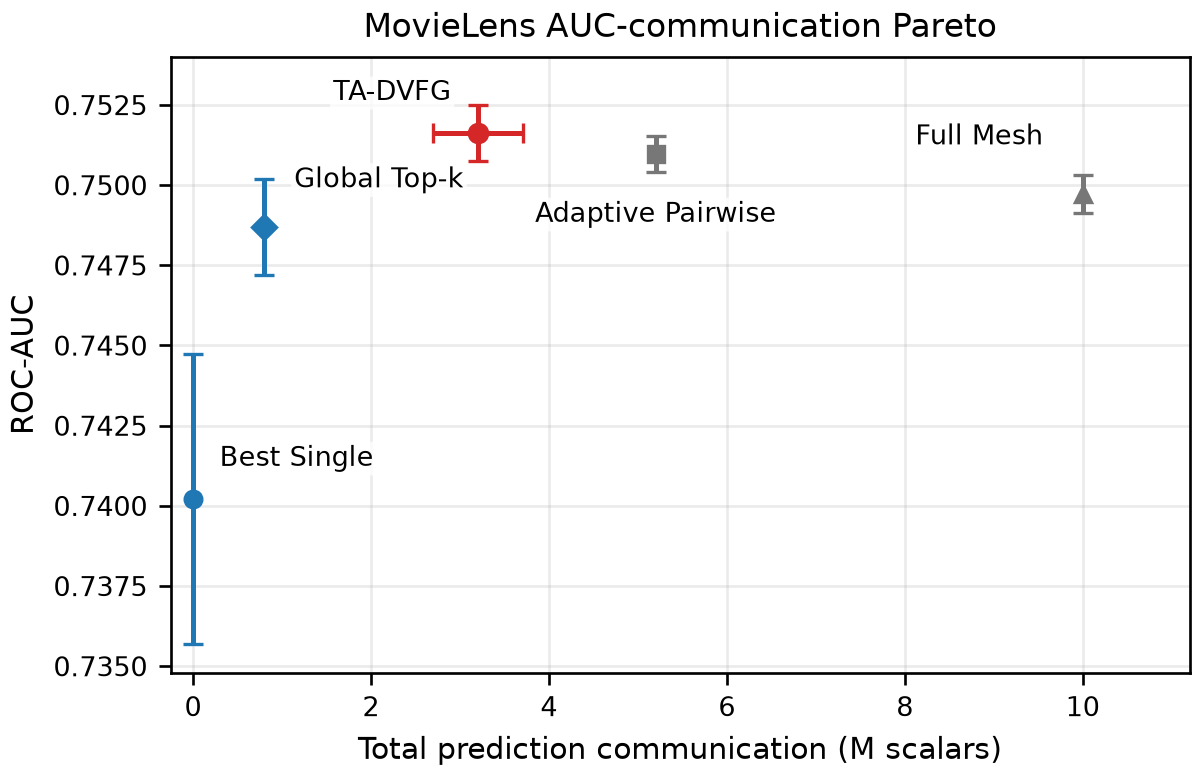
\includegraphics[width=0.37\textwidth]{figures/movielens_pareto_auc_communication.png}
\hfill

\includegraphics[width=0.43\textwidth]{figures/movielens_party_val_test_auc.png}
\caption{MovieLens evidence. Left: AUC--communication trade-off
(Table~\ref{tab:movielens-main}A). Right: validation/test AUC of heterogeneous
local predictors.}
\label{fig:movielens-evidence}
\end{figure*}


\paragraph{MovieLens real-data heterogeneous predictor evaluation.}
The five parties span interaction, profile, temporal, metadata, and genre views
using MF, MLP, and KNN+MLP predictors with parameter counts
651,970/130,402/162/825,218/297,938.
Figure~\ref{fig:movielens-evidence} shows standalone predictor variation and
the AUC--communication trade-off. Best Single reaches 0.7402 AUC with zero communication; seed-level deltas
appear in the supplement.

Table~\ref{tab:movielens-main} shows that \method{} reaches 0.7516 ROC-AUC with 3.20M communication,
compared with 0.7497/10.00M for Full Mesh and 0.7510/5.20M for Adaptive
Pairwise. Because the absolute AUC differences are small, the main five-party result is one of Pareto efficiency rather than a large predictive gain:
\method{} uses 68.0\% less communication than Full Mesh and 38.5\% less than
Adaptive Pairwise. In the controlled 15-party Main and Hard stress settings,
\method{} reaches 0.7516/0.7498 AUC with 5.2/5.0 links, outperforming 105-link
Full Mesh and Adaptive Pairwise with roughly 14 links. When many weak predictors
are present, selective graph construction therefore provides both sparsity and
a predictive benefit.

\paragraph{Cross-benchmark interpretation.}
In MovieLens-5, topology learning mainly improves Pareto efficiency, whereas
under weak-predictor stress it also improves robustness by filtering harmful
communication.

\paragraph{Stronger-information latent-alignment references.}
The main method does not assume access to a shared latent interface. Direct
latent-alignment methods therefore require a stronger information boundary:
they collect genuine hidden states and learn a shared projection or fusion
module.

We ran a separate five-seed ACM Hard reference suite in which all methods
within each seed used the same freshly trained and subsequently frozen local
predictors. Historical
headline caches were excluded because a comparability audit found different
predictor realizations. Hidden-state export reproduced the original forward path
exactly in all 75 party--seed checks. All-party Project-and-Mean reaches
$59.41\pm1.51\%$, and validation-reliability selection raises it to
$77.10\pm0.93\%$. On the same frozen predictors, \method{} reaches
$85.60\pm1.16\%$, exceeding the selected latent reference by 8.50 percentage
points (95\% CI $[6.54,10.47]$, paired $t$-test
$p=2.76\times10^{-4}$; \method{} win/tie/loss: 5/0/0).

A useful-party-only latent-fusion oracle reaches $88.93\pm0.94\%$, showing that
latent fusion itself can be strong when useful parties are known. The deployable
challenge is instead identifying and combining useful parties among many weak
predictors. We therefore treat these methods as centralized
stronger-information references rather than communication-matched P2P
baselines, and we do not claim universal superiority over all latent-alignment
interfaces.

\begin{figure*}[!t]
\centering
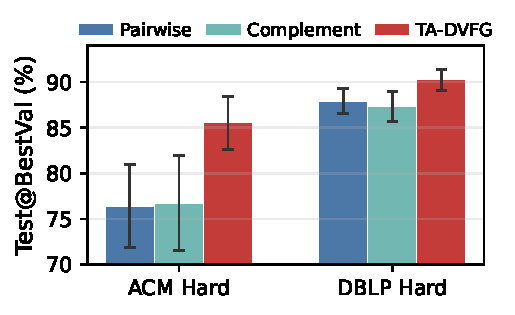
\includegraphics[width=0.36\textwidth]{figures/topology_objective_ablation.pdf}
\hfill
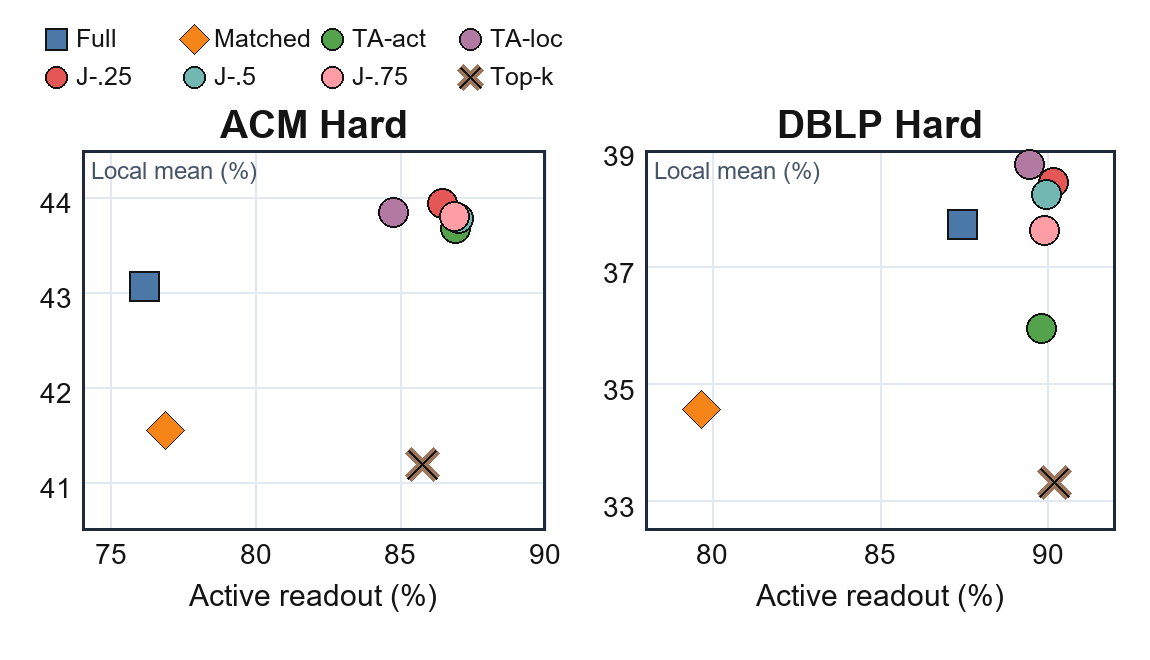
\includegraphics[width=0.41\textwidth]{figures/deployment_tradeoff.png}
\caption{Mechanism and deployment. Left: graph-level versus pairwise and
complementarity-only selection. Right: active/local trade-offs across deployment
objectives.}
\label{fig:mechanism-deployment}
\end{figure*}

\paragraph{Mechanism and deployment analysis.}
Figure~\ref{fig:mechanism-deployment} shows graph-level selection at
85.54/90.25\% on ACM/DBLP Hard, versus 76.41/87.91\% for Adaptive Pairwise
and 76.74/87.32\% for Adaptive Complementarity. Table~\ref{tab:active-only-boundary}
shows that subset selection slightly exceeds active-only readout at lower cost.
Disabling only peer exchange changes active accuracy by at most 0.20 points but
reduces all-party local mean by 1.85/2.67 points and connected-party accuracy
by 4.79/7.16 points. Thus active-only deployment is mainly participant
selection, whereas local or joint deployment is where peer exchange adds a
distinct capability.

\paragraph{Label ownership and deployment readouts.}
Under the label-location protocol, only the active party receives training and
validation labels; passive parties submit logits and receive logit-space
gradients. On ACM and DBLP Hard, the joint-0.25 objective reaches
86.43/90.15\% active readout and 43.94/38.45\% all-party local mean with only
5.0/6.0 links, outperforming Full Mesh on both interfaces. Global Top-$k$
remains slightly stronger on DBLP active readout but is weaker on local
consensus. This protocol separates label location but does not guarantee label
confidentiality.

\paragraph{Efficiency and robustness.}
Using only 10\% of topology-validation labels yields 87.02/89.83\% on ACM and
DBLP Hard, close to 86.99/90.25\% with the full validation split, while
reducing topology-collection traffic by about 90\%. Updating every 50 epochs
performs comparably to the 20-epoch default while reducing topology-selection
communication by 60\%.

Two further stress tests support the topology interpretation. Across
$K\in\{1,2,3\}$, \method{} remains stable at
85.54/85.17/85.83\% on ACM Hard and 90.25/90.15/90.34\% on DBLP Hard,
while mean reachable parties increase from 1.67 to 2.31/2.15, respectively.
We therefore retain $K=1$ as the lower-communication default. In nested
3--18-party scaling with three useful predictors fixed, the
\method{}--Full Mesh gap widens from zero to 12.59/5.16 percentage points
on ACM/DBLP as 15 weak predictors are added, while \method{} retains about
five links versus 153 for Full Mesh.

From 5 to 30 parties, candidate evaluations rise from 617 to 41,542 and
topology time from 0.81 to 81.46 seconds while selected graphs stay near five
links, confirming exhaustive scoring as the current bottleneck. Minimum-link
and edge-budget sweeps show that nonempty sparse collaboration emerges without
a minimum quota: with $m=0$, every ACM/DBLP Hard seed selects a nonempty graph
(2.6/3.0 edges on average), with DBLP unchanged and ACM higher in this sweep;
beyond any minimum quota, $B$ remains an upper bound; full results appear in
the supplement.



\section{Discussion}

Global Top-$k$ and same-cardinality subset selection are strong centralized
choices for active-only deployment. \method{} is most justified when deployment
also requires party-local predictions, because its sparse links materially
improve connected parties.

The latent-alignment study sharpens this interface distinction. Weak parties
hurt naive all-party fusion, while validation-based selection recovers much of
the loss; the useful-party oracle shows latent fusion itself can be strong. The
question is therefore which information interface and selection mechanism are
available at deployment. On ACM Hard, \method{} remains above the deployable
reliability-selected latent reference while using only task-level outputs and
producing a sparse peer graph.

Edge identities are too unstable for a semantic ``discovered relationship''
claim. With $K=0$, mean edge-set Jaccard is 0.410/0.164 on ACM/DBLP Hard;
removing degree weighting reproduces the same topology in only 1/10 runs, yet
active utility changes little. We call this \emph{utility stability under
structural multiplicity}: distinct sparse graphs can be near-equivalent for the
current predictors and objective. The graph is a deployment artifact, not a unique structure.

\section{Limitations and Conclusion}

Several limitations remain. First, for active-only deployment, direct subset
selection matches or slightly exceeds \method{} in mean accuracy at lower
communication on the audited Hard settings. The learned graph is therefore most
valuable when party-local inference is also required. Second, reducing the
collaboration interface to predictions does not provide a privacy guarantee:
predictions, validation signals, and optional logit gradients may still leak
information. Compatible output semantics also do not ensure identical
calibration across predictors, and the current reliability weighting does not
explicitly calibrate per-party distributions. Third, HGB provides controlled
graph-view constructions, while
MovieLens-5 uses real recommendation data with constructed heterogeneous party
interfaces rather than a naturally occurring five-organization federation; the
15-party MovieLens settings are controlled weak-predictor stress tests.

Fourth, the direct latent-alignment study is limited to ACM Hard with frozen
local predictors. It shows that reliability-selected latent fusion remains below
\method{} in this setting, while the useful-party-only oracle shows that stronger
hidden-state fusion can be effective when useful parties are known. Broader
multi-dataset and end-to-end alignment studies therefore remain future work.
Finally, nested weak-party scaling shows that \method{}'s advantage over
dense and edge-local P2P methods widens as controlled weak predictors are
added. This trend should not be extrapolated to naturally occurring parties
or to architectural heterogeneity, for which we do not establish a monotonic
relationship. Because the primary results use only five seeds, non-significant paired
tests should not be interpreted as evidence of equivalence.

Sparse deployment communication scales with the selected edge set, but
exhaustive candidate scoring remains the current scalability bottleneck. A
concrete next step is two-stage screening: use a cheap edge-local score to
shortlist the top-$M$ feasible candidates, then apply the existing whole-graph
rerun only to that shortlist. We do not report a pruning result here, so its
accuracy--time trade-off remains an open experiment rather than a claimed
contribution.

All source code required to conduct and analyze the reported experiments will be
released publicly upon publication; the review package contains the referenced
analysis scripts and raw outputs. Exact hardware and software-version metadata
are only partially preserved in the current artifact and remain a
reproducibility limitation.

In summary, \method{} reframes vertical graph-view collaboration as sparse
prediction-space deployment. Prediction space determines what heterogeneous
predictors can share; deployment requirements determine whether collaboration
needs only participant selection or a learned peer topology. Direct subset
selection is a strong active-only alternative, whereas sparse peer exchange
materially improves party-local predictions. Future work should protect
exchanged messages, scale topology search, and further characterize the
performance--interface trade-off between prediction-space peer deployment and
stronger-information latent fusion.

\bibliography{references}
\end{document}



